\section{Miscellaneous}
\label{sec:miscellaneous}
In this section three relevant works for the state of the art are treated.
Their contributions can be briefly summed up like this:
\begin{enumerate}
	\item{MiDaS makes it possible to train on heterogeneous datasets.}
	\item{PatchFusion allows predicting high-resolution depth maps.}
	\item{Marigold proves the effectiveness of pre-trained vision foundation models and synthetic data in this domain.}
\end{enumerate}

%%%%%%%%%%%%%%%%%%%%%%%%%%%%%%%%%%%%%%%%%
%              MiDas
%%%%%%%%%%%%%%%%%%%%%%%%%%%%%%%%%%%%%%%%%
\subsection{MiDaS}
MiDaS \cite{MiDas} is a technique for training depth estimation models on multiple datasets.
It was encountered in various works discussed in here.
The main depth estimation datasets are not sufficiently rich to train a robust model resulting in poor generalization and poor transferability to other datasets and to unconstrained scenes.
MiDas, which stands for "Mixing Datasets", is a technique for training a depth estimation model on diverse labeled data by using a loss function that is invariant to the various differences among datasets.
The authors of \cite{MiDas} also used 3D-movies as a source of stereo data and, they did a great work in cleaning it up and converting it to suitable disparity maps.
When working with different datasets simultaneously, three main incompatibilities arise:
\begin{enumerate}
	\item Ground truth representation, which can be a depth map or a disparity map
	\item Scale ambiguity, some datasets use relative depth and others provide up-to-scale depth maps
	\item Shift ambiguity, 3D movies stereo pairs in particular present a global disparity shift.
\end{enumerate}
First: they choose to work in disparity space.
Then, when comparing a ground truth disparity map $\mathbf{D}^{*}$ and a predicted disparity map $\mathbf{D}$ they scale and shift the two so that they have zero shift and unit scale.
They approximate the idea of "scale" and "shift" by means of two functions $s$ and $t$:
\[
	t(\mathbf{D}) := \mathop{\text{median}}_{p \in \mathbf{D}}(\mathbf{D}(p))
\] \[
	s(\mathbf{D}) := \mathop{\text{mean}}_{p \in \mathbf{D}} \big| \mathbf{D}(p) - t(\mathbf{D}) \big|
\] \[
	\hat{\mathbf{D}} = \frac{\mathbf{D} - t(\mathbf{D})}{s(\mathbf{D})}
\] \[
	\hat{\mathbf{D}}^{*} = \frac{\mathbf{D}^{*} - t(\mathbf{D}^{*})}{s(\mathbf{D}^{*})}
\]
Finally their scale and shift invariant ($ssi$) loss is:
\[
	\mathcal{L}_{ssi} = \mathop{\text{mean}}_{p \in \mathbf{D}} \big| \hat{\mathbf{D}}(p) - \hat{\mathbf{D}}^{*}(p)\big|
\]
They regularize it using the following term, which biases the prediction discontinuities to match the ones in the respective ground truth:
\[
	\mathcal{L}_{reg} = \mathop{\text{mean}}_{p \in \mathbf{D}}
		\left(
			\big| \partial_{x} (\hat{\mathbf{D}} - \hat{\mathbf{D}}^{*}) \big| +
			\big| \partial_{y} (\hat{\mathbf{D}} - \hat{\mathbf{D}}^{*}) \big| 
		\right)(p)
\]
Lastly, it is discussed which mixing strategies to use for sampling the datasets in the mini-batches of the stochastic gradient descent algorithm.
Ranftl et al., the authors, propose to use a Pareto-optimal strategy from \cite{pareto}.
This mixing-strategy is often used by works citing this paper, while the scale and shift invariant loss introduced is often replaced by the scale-invariant loss from \cite{Eigen}.

For testing the obtained model, some datasets are put aside so that the zero-shot capability (i.e. how good the model is on completely new data) can be investigated using the experimental protocol called \textit{zero-shot cross-dataset transfer}.

The model architecture trained with this Mixing Datasets strategy is an encoder-decoder as in \cite{ReDWeb}.

%%%%%%%%%%%%%%%%%%%%%%%%%%%%%%%%%%%%%%%%%
%              PatchFusion
%%%%%%%%%%%%%%%%%%%%%%%%%%%%%%%%%%%%%%%%%
\subsection{PatchFusion}
\label{subsec:patchfusion}
Li et al. \cite{PatchFusion} address the problem of metric monocular depth estimation for high-resolution inputs.
Their method, PatchFusion, aligns with so called \textit{Tile-Based Methods}.
In here only this tile-based method is discussed.

% architecture
\begin{figure}
	\centering
	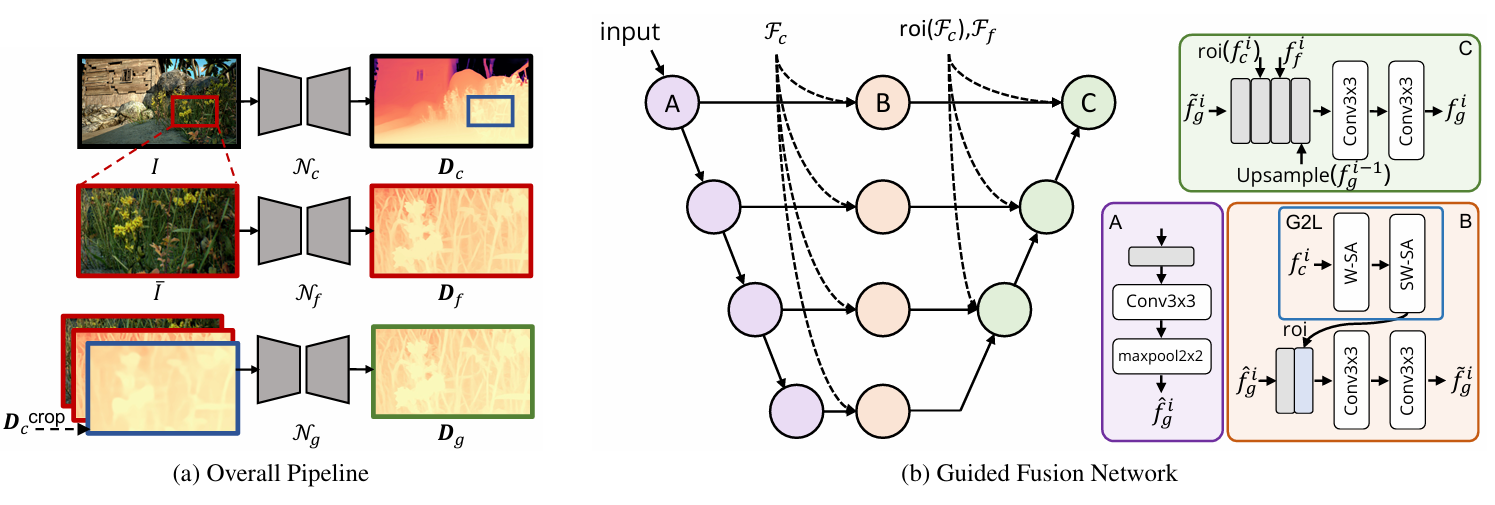
\includegraphics[scale=0.3]{figs/patchfusion}
	\caption{Li et al. architecture \cite{PatchFusion}. \label{fig:patchfusion}}
\end{figure}

The architecture employed (see figure \ref{fig:patchfusion}) is composed of three networks:
\begin{enumerate}
	\item{a global-scale aware prediction network which takes as input a high-resolution down-sampled image and outputs a coarse depth map;}
	\item{a patch-wise depth prediction network which takes as input an image patch and outputs its fine relative depth map;}
	\item{a guided-fusion network.}
\end{enumerate}
The guided-fusion network is quite intricate, but its role is simply to further process the fine depth map of a patch to make it scale-aware.
It takes as inputs the fine depth map patches and crops of the original image and of its estimated coarse depth map corresponding to those patches.
The idea is that while each fine depth map patch has a correct relative depth, when merging them together they need to be aligned with the depth values.
The predicted coarse map defines the scale of the whole final prediction to which patches are aligned to.
With this machinery is now possible to divide a high-resolution image in patches and compute a depth map for each patch, covering the whole image and obtaining a full depth map, but patch artifacts are yet to be removed.
To this end \textit{Consistency-Aware Training} is performed by subdividing the images in overlapping patches and minimizing also the agreement between the patch depth maps and feature maps.
If $\mathbf{Z}_{1}$ and $\mathbf{Z}_{2}$ are two overlapping patch depth maps and $\mathbf{F}_{1}$, $\mathbf{F}_{2}$ their respective feature maps, the consistency-aware loss term is:
\[
	\mathcal{L}_{consistency} =
		\mathop{\text{mean}}_{p \in \mathbf{F}_{1} \cap \mathbf{F}_{2}}
		\left(
			\big\| \mathbf{F}_{1}(p) - \mathbf{F}_{2}(p) \big\|_{2} + \mu \big| \mathbf{Z}_{1}(p) - \mathbf{Z}_{2}(p) \big|
		\right)
\]
Where $\mu$ is a hyperparameter.
One important technical detail of their guided-fusion network is that SwinTransformer layers \cite{swin} are used to process feature maps and preserve global context \cite{PatchFusion}.

%%%%%%%%%%%%%%%%%%%%%%%%%%%%%%%%%%%%%%%%%
%              Marigold
%%%%%%%%%%%%%%%%%%%%%%%%%%%%%%%%%%%%%%%%%
\subsection{Marigold}
Ke et al. \cite{Marigold} prove that a comprehensive representation of the visual world is the cornerstone of (relative) monocular depth estimation.
Their insight is to use priors learned by generative diffusion models to enable more generalizable depth estimation, in particular they adopt Stable Diffusion v2 \cite{StableDiffusionV2} pretrained Variational Auto Encoder(VAE) and Latent Diffusion U-Net.
The overall pipeline is shown in figure \ref{fig:marigold}.

% architecture
\begin{figure}
	\centering
	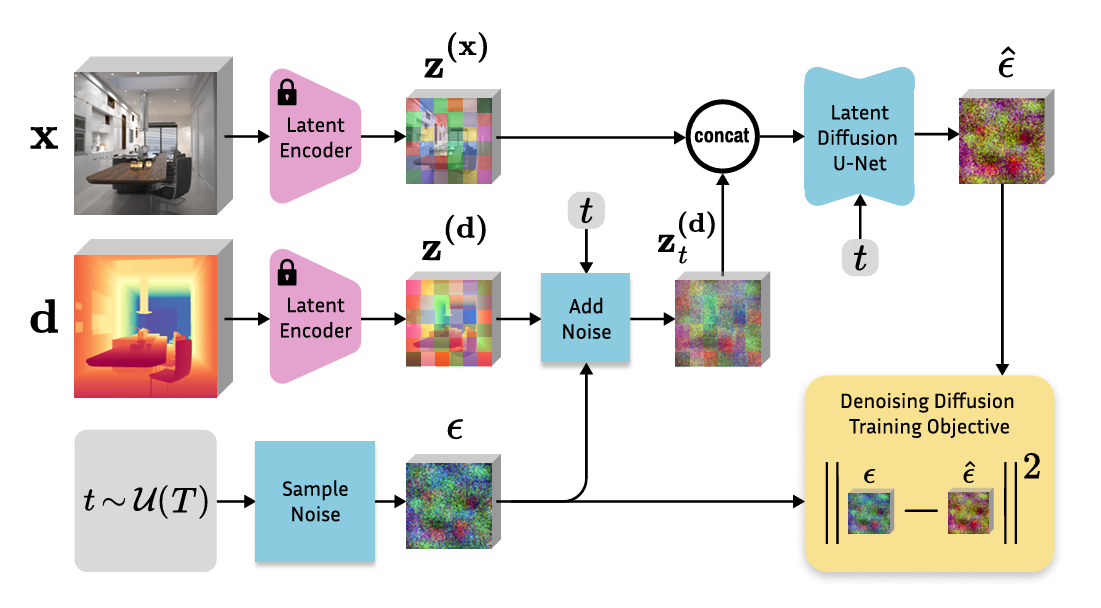
\includegraphics[scale=0.3]{figs/marigold}
	\caption{Ke et al. architecture as illustrated in their paper \cite{Marigold}. \label{fig:marigold}}
\end{figure}

Monocular depth estimation is here posed as a conditional denoising diffusion generation task.
The idea is to teach a model called "diffusion model" to clean a depth map from noise conditioned to the corresponding RGB image.
More formally consider an RGB image $\mathbf{I}$, its depth map $\mathbf{Z}^{*}$ and its noise corrupted depth map $\tilde{\mathbf{Z}}_{0}$ (which can be so corrupted to be just sampled random noise, i.e. $\mathbf{Z}$ needn't be known), the diffusion model takes as input the two and outputs a less noisy depth map $\tilde{\mathbf{Z}}_{1}$.
The noise is modeled as additive, hence:
\[
	\tilde{\mathbf{Z}}_{1} = \tilde{\mathbf{Z}}_{0} + \epsilon(\mathbf{I}, \tilde{\mathbf{Z}}_{0})
\]
where $\epsilon$ is the computed noise to remove.
After iteratively repeating the procedure a few times the resulting depth map is expected to match the ground truth depth map: $\tilde{\mathbf{Z}}_{T} \approx \mathbf{Z}^{*}$ for $T$ large enough.
Actually, all this process takes place in a \textit{latent space}, meaning that instead of working with depth maps and images, the diffusion model works with their lower dimensional representations computed by the encoder $\mathcal{E}$ from the pretrained Stable Diffusion VAE(and with fixed parameters) and noise is added in that space.
For getting the final depth estimate the decoder $\mathcal{D}$ from the same VAE is used.

I'm not giving all the details here, but one thing to know is how a pretrained model that works with RGB images can work with depth maps: depth maps are first affinely trasformed to be in approximately the range $[-1, +1]$ and then are replicated into three channels.
In this way they are compatible with the Stable Diffusion VAE which outputs a three channel tensor.
Nevertheless, it is not obvious at all that the VAE alone can reconstruct this kind of image, but Ke et al. experimentally observed that $\mathbf{Z} \approx \mathcal{D}(\mathcal{E}(\mathbf{Z}))$ with a negligible error.
Another remarkable fact is that Marigold is trained only on synthetic data and generalizes so well to real world data that beats various other methods in almost every unseen test dataset they evaluated the model on.